\documentclass[a4paper,10pt,fleqn]{jarticle}
\usepackage[top=30truemm,bottom=30truemm,left=27truemm,right=27truemm]{geometry}
\usepackage[dvipdfm]{graphicx}
\usepackage{here}
\usepackage{listings}
\begin{document}
%%%%%
\begin{titlepage}
\begin{center}
\vspace*{150truept}
{\Huge 情報可視化論 最終課題解説}\\ % タイトル
\vspace{10truept}
%{\huge ―サブタイトル―}\\ % サブタイトル(なければコメントアウト)
\vspace{200truept}
{\Large 学籍番号 179X005X}\\ % 学籍番号
\vspace{20truept}
{\Large 川西 亮平}\\ % 著者
\vspace{20truept}
{\Large 提出日:\today}\\ % 提出日
\end{center}
\end{titlepage}
%%%%% 本文ここから %%%%%%
\section{解説}
最終課題は12週目の課題に機能を追加したものになります.作成したファイルの全体図はFig. \ref{全体図}のようになり,追加したUI部分を拡大した図はFig. \ref{UI}のようになります.追加した機能は(a)Isovalueの変更,(b)カラーマップの切り替え,(c)シェーディング表示のオン・オフ切り替えの3つになります.それぞれの機能について以下で説明します.
\begin{figure}[H]
\renewcommand{\figurename}{Fig.}
\begin{center}
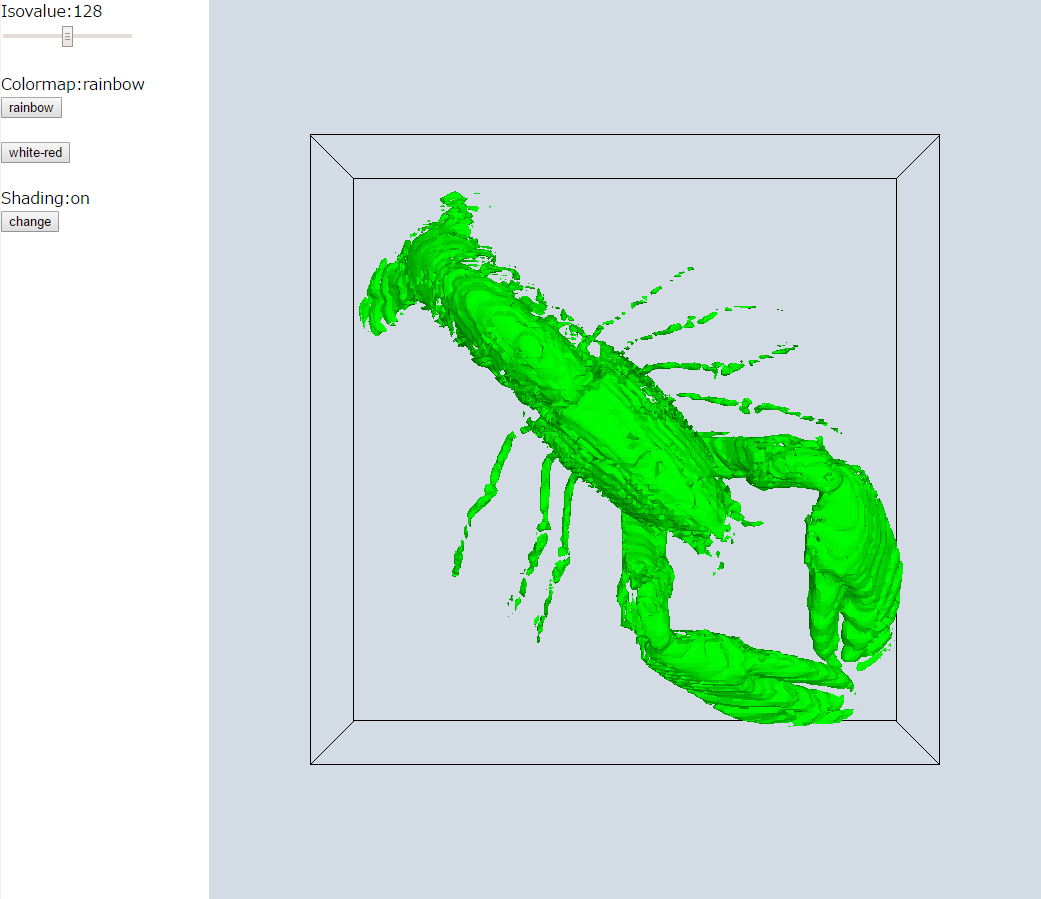
\includegraphics[width=14cm,bb=0 0 1041 899]{全体図.png}
\caption{全体図}
\label{全体図}
\end{center}
\end{figure}
\begin{figure}[H]
\renewcommand{\figurename}{Fig.}
\begin{center}
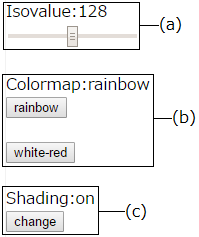
\includegraphics[width=4cm,bb=0 0 199 237]{UI.png}
\caption{追加したUI}
\label{UI}
\end{center}
\end{figure}
\subsubsection*{(a) Isovalueの変更}
この部分は,Isovalueの値を変化させるためのスライダである.スライダの最小値は0,最大値は255,間隔は1で初期値は128となっています."Isovalue:"の横の値は現在のIsovalueの値を表しており,スライダを動かすと変化します.(b),(c)の部分のボタンを押すことで現在のIsovalueの値で表示します.Fig. \ref{全体図}の状態からIsovalueを81にしたときの全体図はFig. \ref{isovalue}となります.
\subsubsection*{(b) カラーマップの切り替え}
この部分は,カラーマップを切り替えるためのボタンである.上の"rainbow"ボタンを押すことで虹色カラーマップに,下の"white-red"ボタンを押すことで白赤カラーマップに切り替え表示します.初期状態では虹色カラーマップになっています."Colormap:"の横は現在使用されているカラーマップを表示します.虹色カラーマップの場合は"rainbow"を,白赤カラーマップの場合は"white-red"を表示します.Fig. \ref{全体図}の状態から白赤カラーマップに切り替えたときの全体図はFig. \ref{white-red}となります.
\subsubsection*{(c) シェーディング表示のオン・オフ切り替え}
この部分は,シェーディング表示のオン・オフを切り替えるためのボタンである."change"ボタンを押すとシェーディング表示がオンの場合はオフに,オフの場合はオンに切り替えます.初期状態ではシェーディング表示はオンになっています."Shading:"の横は現在シェーディング表示されているかを表示します.Fig. \ref{全体図}の状態からシェーディング表示をオフに切り替えたときの全体図はFig. \ref{shading}となります.
\begin{figure}[H]
\renewcommand{\figurename}{Fig.}
\begin{center}
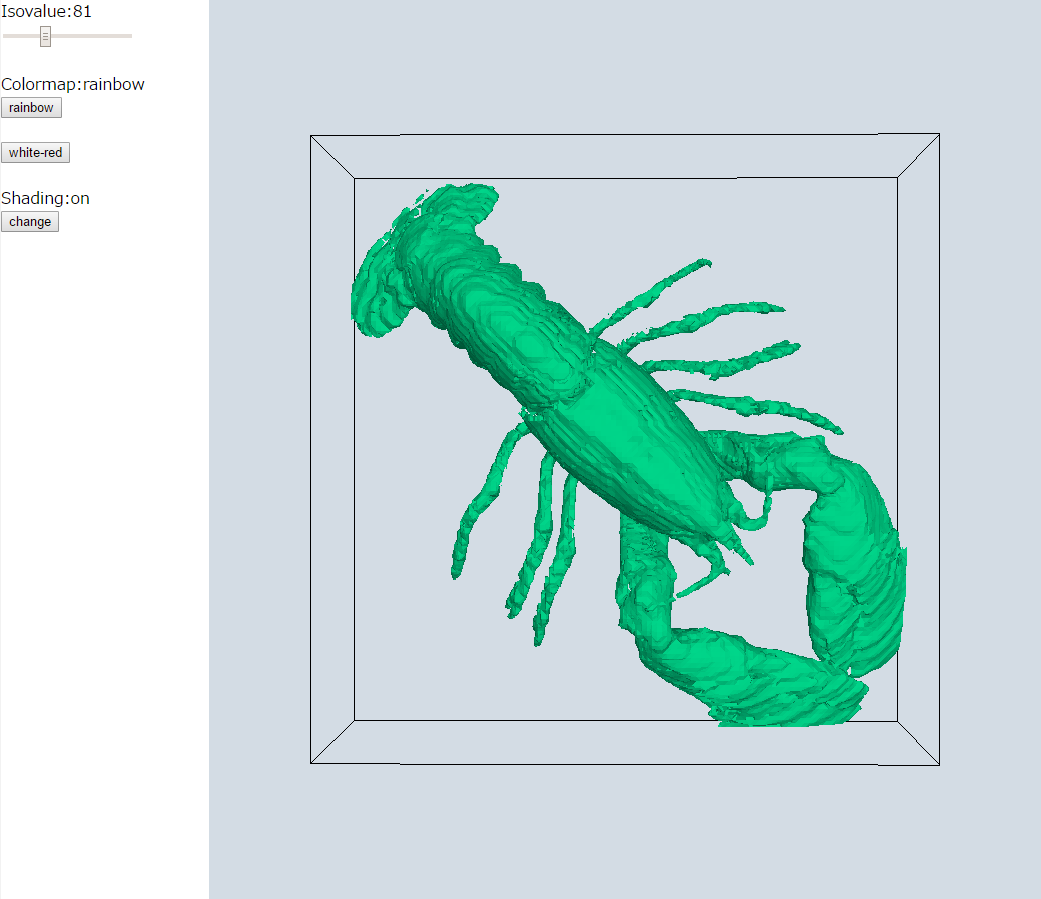
\includegraphics[width=10cm,bb=0 0 1041 899]{Isovalue.png}
\caption{Isovalue=81のときの全体図}
\label{isovalue}
\end{center}
\end{figure}
\begin{figure}[H]
\renewcommand{\figurename}{Fig.}
\begin{center}
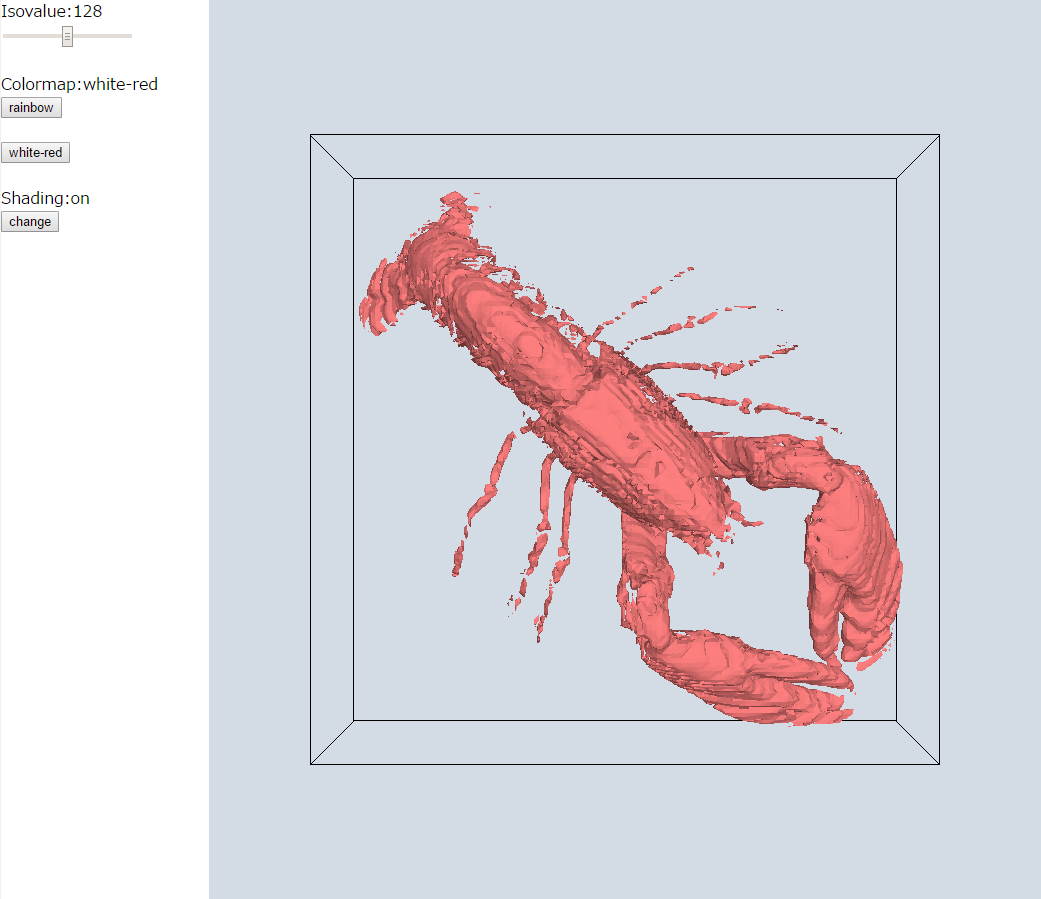
\includegraphics[width=10cm,bb=0 0 1041 899]{white-red.png}
\caption{白赤カラーマップのときの全体図}
\label{white-red}
\end{center}
\end{figure}
\begin{figure}[H]
\renewcommand{\figurename}{Fig.}
\begin{center}
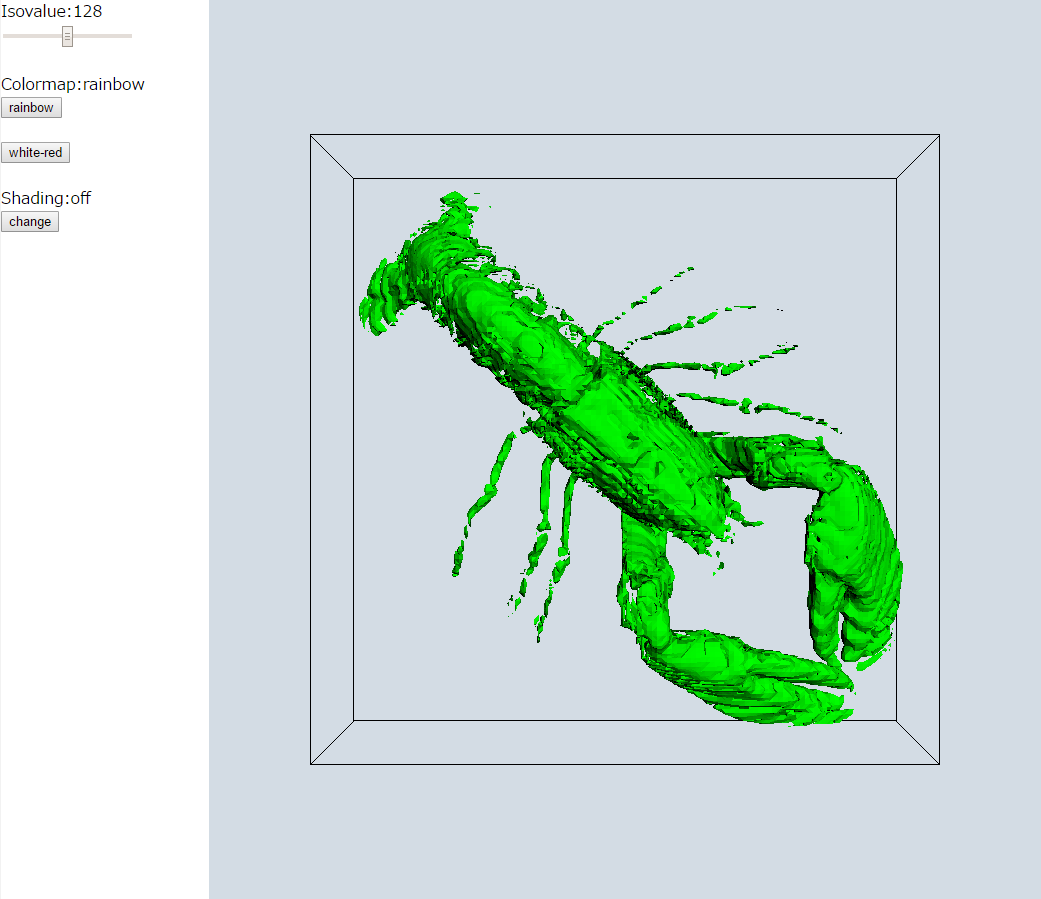
\includegraphics[width=10cm,bb=0 0 1041 899]{shading.png}
\caption{シェーディング表示オフのときの全体図}
\label{shading}
\end{center}
\end{figure}
%\lstset{
%    frame=single,
%    numbers=left,
%    tabsize=2
%}
%\begin{lstlisting}[label=src1, caption=Pythonのコード]
%<html>
%    <head>
%	<title>Final Task</title>
%\end{lstlisting}
\end{document}